\section{Introdução}


\begin{frame}{Dados nunca dormem}
    \begin{figure}[h!]
        \centering
        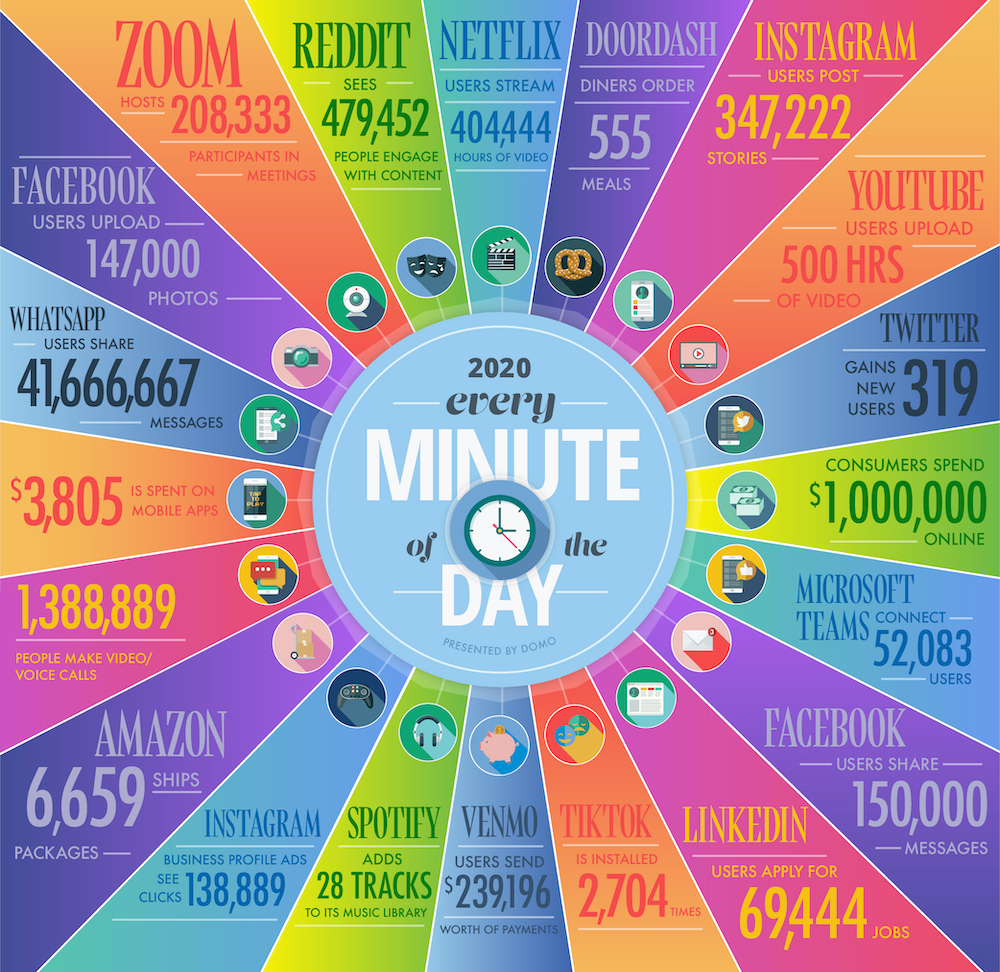
\includegraphics[scale=0.75]{images/data-never-sleeps.jpg}
        
        \caption{Infográfico: Data Never Sleeps 8.0 }
        \footnotesize{Fonte: \cite{data-never-sleeps}}
    \end{figure} 
\end{frame}

\begin{frame}{Aumento na produção de dados}
	\begin{figure}[h!]
        \centering
        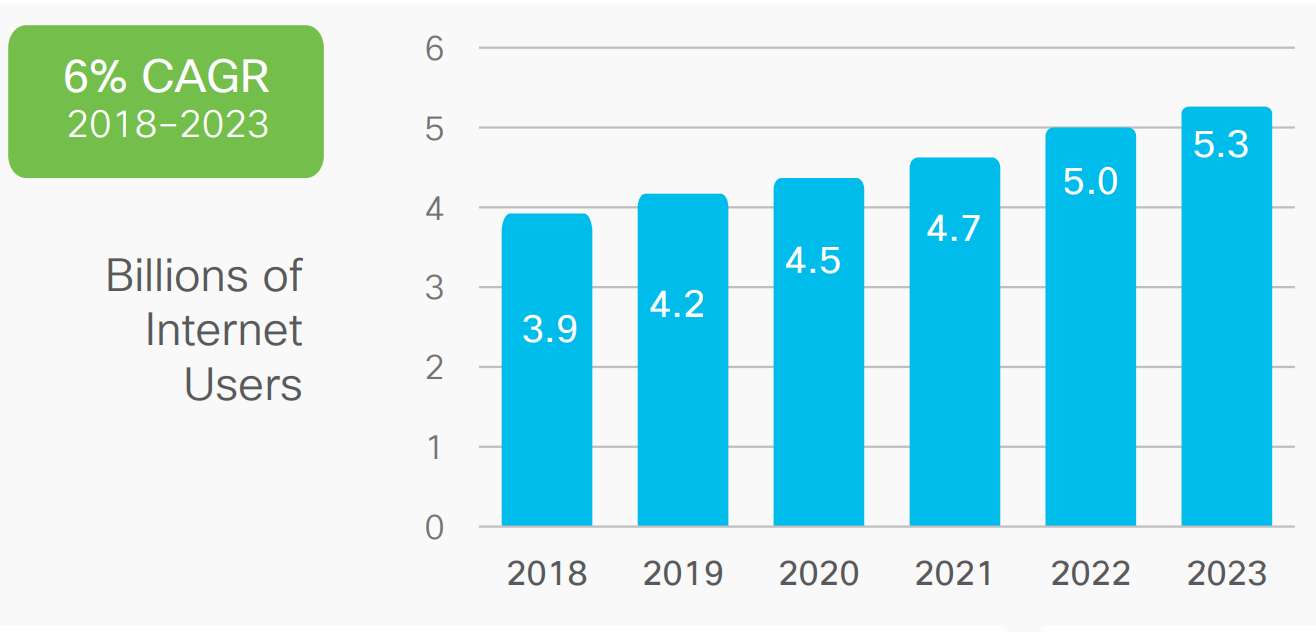
\includegraphics[scale=0.2]{images/relatorio-cisco.png}
        
        \caption{Número de usuários conectados à internet}
        \footnotesize{Fonte: \cite{report-cisco}}
    \end{figure} 
\end{frame}


\begin{frame}{Aumento na produção de dados}
	\begin{figure}[h!]
        \centering
        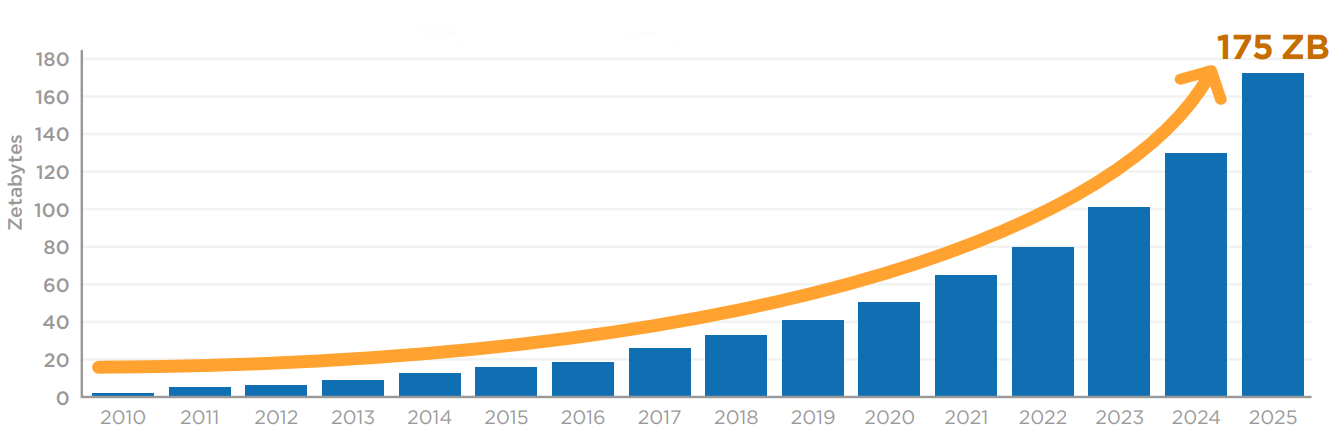
\includegraphics[width=\columnwidth]{images/relatorio-idc.png}
        
        \caption{Esfera global de dados por ano}
        \footnotesize{Fonte: \cite{relatorio-idc}}
    \end{figure} 
\end{frame}

\begin{frame}{Segmentação da indústria e Gargalo de Von-Neumann}
	\begin{figure}[h!]
        \centering
        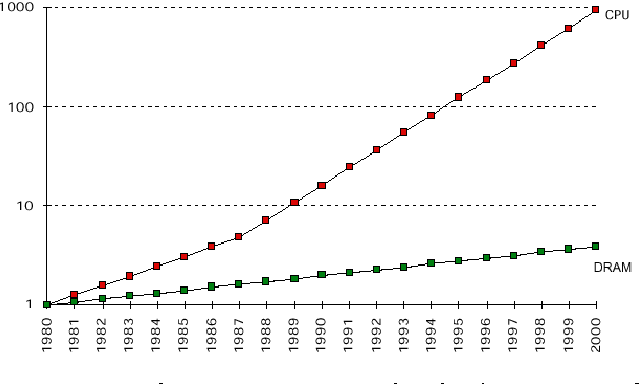
\includegraphics[scale=0.42]{images/gap-processor-memory.png}
        
        \caption{Lacuna de desempenho entre processador e memória}
        \footnotesize{Fonte: \cite{fig-gap-processor-memory}}
    \end{figure} 
\end{frame}

\begin{frame}{Hierarquia de memória}
	\begin{figure}[h!]
        \centering
        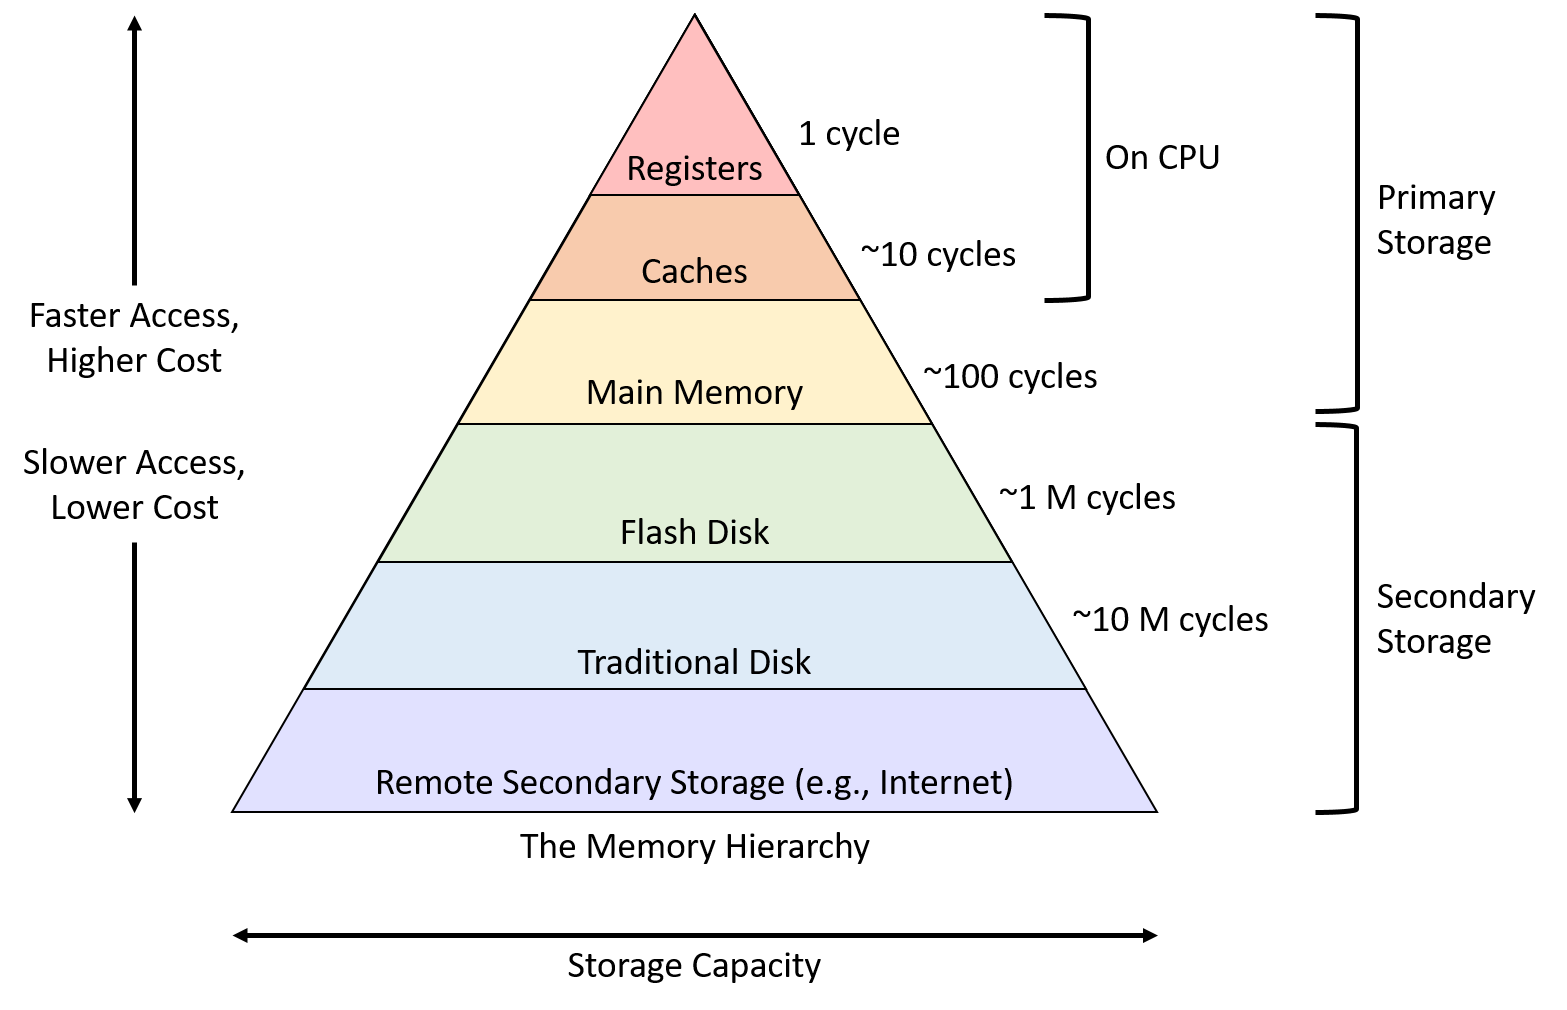
\includegraphics[scale=0.3]{images/hierarquia-memory-2.png}
        
        \caption{Hierarquia de memória}
        \footnotesize{Fonte: \cite{paper-gap-between-processor-memory}}
    \end{figure} 
\end{frame}

\begin{frame}{Hierarquia de memória}
	\begin{figure}[h!]
        \centering
        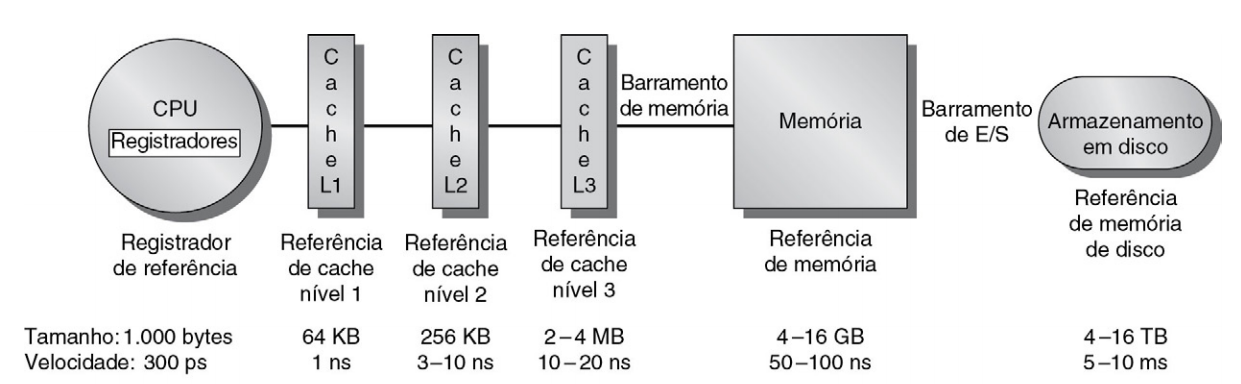
\includegraphics[width=\columnwidth]{images/hierarquia-memory.png}
        \caption{Hierarquia de memória de um servidor}
        \footnotesize{Retirado de: \cite{book-computer-architecutre}}
    \end{figure} 
\end{frame}

\begin{frame}{Solução}
    \begin{itemize}
        \item Atuar nos níveis com menor latência;
        \item Estrutura de dados e compactação de dados:
        \begin{itemize}
            \item Representação do DNA através de árvore de sufixos;
            \item Compressão de dados clássica vs Estrutura de dados sucintas.
        \end{itemize}
    \end{itemize}
\end{frame}

\begin{frame}{Proposta}
    \begin{itemize}
        \item \cite{paper-fully-functinal-succint-trees}, range min-Max tree (rmM-tree);
        \item Um novo gargalo;
        \item range min-Max k-ária.
    \end{itemize}
\end{frame}